\begin{table}[t]
\centering
\caption{Shortcut probes. Macro AUROC on all \NImages{} images and on the \NMixed{} images from the
two case repositories that contain \emph{both} COVID-19 and non-COVID cases (Radiopaedia,
Eurorad), where the source cannot identify the label. Logistic regressions use the same folds.}
\label{tab:reference}
\small
\setlength{\tabcolsep}{4pt}
\begin{tabular}{@{}lcc@{}}
\toprule
Model & all images & mixed-source subset\\
\midrule
\tabinput{tables/reference.tex}
\bottomrule
\end{tabular}
\end{table}

\paragraph{Diagnosis terms in notes.} \PctMasked\% of the notes name the diagnosis or the
pathogen. Leaving these terms unmasked raises note + structured from \AUC{txt_tab_only} to
\AUC{txt_tab_only_rawtext} and IRENE from \AUC{irene_k2} to \AUC{irene_k2_rawtext}
(\cref{fig:robust}a). The gain is smaller than one might expect, because the remaining text is
itself highly predictive. A TF-IDF logistic regression on the \emph{masked} notes reaches
\CL{tfidf_masked}, almost as high as on raw notes (\CL{tfidf_raw}), and above every transformer
in this study (\cref{tab:reference}). Masking is still necessary for a fair evaluation, but it is
far from sufficient.

\paragraph{Source confounding.} Public COVID-19 collections gather cases from sources that
differ systematically in their label mix. Some are almost entirely COVID-19 (the SIRM archive,
GitHub-hosted hospital releases, NEJM case reports), while others are mostly non-COVID
(Eurorad). A logistic regression that sees \emph{only} the host of the source URL reaches
\CL{source_only} macro AUROC, on par with the fusion transformers. The notes and the view
(\CL{view_only}) carry this signal implicitly through writing style, translation artefacts
and acquisition protocol. As a de-confounded check, we recompute every metric on the \NMixed{}
images from Radiopaedia and Eurorad, the two repositories that host both COVID-19 and
non-COVID cases. There the source-only probe falls to chance (\CL{source_only@mixed}). The fused models
lose about 6 points and the image-only model about 3, but the ranking is preserved (\cref{tab:reference}). Late fusion
(\MIX{late_fusion}), early fusion (\MIX{early_fusion}) and IRENE (\MIX{irene_k2}) remain above
note + structured (\MIX{txt_tab_only}) and image-only (\MIX{img_only}). The TF-IDF note model is
still the strongest (\CL{tfidf_masked@mixed}). This agrees with the radiograph shortcuts reported
by DeGrave et al.\ \citep{degrave2021shortcuts} and argues for reporting a de-confounded subset
alongside headline numbers on public COVID-19 data.

\begin{figure*}[t]
\centering
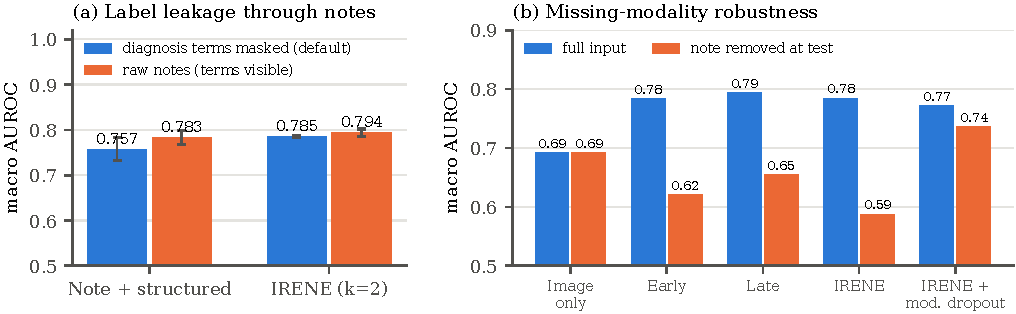
\includegraphics[width=\textwidth]{figures/robustness.pdf}
\caption{(a) Effect of masking diagnosis and pathogen names in the notes (2 seeds for the
raw-note runs). (b) Macro AUROC with the full input and with the note removed at test time.
Modality dropout ($p{=}0.3$) during training closes most of the gap.}
\label{fig:robust}
\end{figure*}

\paragraph{Missing notes.} Deployed systems will not always have a note. When it is removed at
test time, IRENE falls from \AUC{irene_k2} to \NT{irene_k2}, well below the image-only model
(\AUC{img_only}). Early and late fusion degrade less (\NT{early_fusion} and \NT{late_fusion};
\cref{fig:robust}b). The fused models have learned to rely on the note and do not fall back on
the image features. This matches the fragility reported by Ma et al.\ \citep{ma2022missing}.
Training with modality dropout ($p{=}0.3$) raises the no-note AUROC to \NT{irene_k2_moddrop},
close to the image + structured model (\AUC{img_tab}), at a small cost with full input
(\AUC{irene_k2_moddrop}). For a clinical deployment where the note is not always available,
this trade-off is clearly worthwhile.
